\documentclass [11pt,fleqn]{article}

\usepackage{amssymb}
%\usepackage{epsf,psfig,graphicx}
\usepackage{bm}
\usepackage{epsf,graphicx}
\usepackage{psfrag}
\usepackage{amsmath}
\usepackage{color}
\topmargin     -0.60in  % (adjusted for printer bias) 
\headheight      .00in  % (no headers) 
\headsep         .50in  % (top margin + headers + skip) 
\textheight     9.50in  % (instructions: 9 1/8'' min, 9 7/16'' max) 
\textwidth      6.00in  % 2*3.33 + .33 = 6.99 
\oddsidemargin  0.3125in  % (subtracted 1inch bias) 
\evensidemargin 0.3125in 
%\renewcommand{\baselinestretch}{1.5} 
\parindent .0in 
\parskip 10pt 


\font \bigtenrm=cmmi10 scaled\magstep2 
\def \dt {\delta\tau} 
\def \ve {\varepsilon} 
\def \ch {{\cal H}} 
\def \del {\partial} 
\def \be {\begin{equation}} 
\def \ee {\end{equation}} 
\def \beq {\begin{eqnarray}} 
\def \eeq {\end{eqnarray}} 
\def \tv {\tilde v} 
\def \veren {\varepsilon^{\rm ren}_f} 
\def \vef {\varepsilon^0_f} 
\def \su {\uparrow} 
\def \sd {\downarrow} 
\def \CR {\nonumber\\} 
\def \hfb {\hfill\break} 
\def \tb {\bar{t} } 
\def \kb {\bar{k} } 
\def \tbB {\bar{t}_B } 
%\def \ul{#1} {$\underline{#1 }$}

\begin{document} 
\hspace{1cm}{\bf Title:} Observation of correlated x-ray scattering at atomic resolution \hfb
 
{\bf Authors:} Derek Mendez, Thomas J. Lane, Jongmin Sung,  Cl\`ement Levard, Herschel Watkins, Aina Cohen, Michael Soltis, Shirley Sutton, James Spudich, Vijay Pande,  Daniel Ratner, Sebastian Doniach

{\bf Abstract}

Tools to study disordered systems with local structural order, such as proteins in solution, remain limited. Such understanding is essential for \emph{e.g.}~rational drug design. Correlated x-ray scattering (CXS) has recently attracted new interest as a way to leverage next-generation light sources to study such disordered matter. The CXS experiment measures angular correlations of the intensity caused by the scattering of x-rays from an ensemble of identical particles, with disordered orientation and position. Averaging over 15,496 snapshot images obtained by exposing a sample of silver nanoparticles in solution to a micro-focused synchrotron beam, we report an update on experimental efforts to obtain CXS signal from an ensemble in three dimensions. The correlation function was measured at  wide angles corresponding to atomic resolution and matches theoretical predictions. These preliminary results suggest that other CXS experiments on disordered ensembles -- such as proteins in solution -- may be possible in the future.


\section{Introduction}

In a pioneering paper, Kam \cite{Kam:1977wc} showed that correlated x-ray scattering (CXS) from an ensemble of randomly oriented particles could in principle reveal information about the internal structure of the particles beyond usual small and wide angle solution scattering measurements. The extraction of such information in the absence of an ordered system (\textit{e.g.}~a crystal) can be beneficial in biological studies, as many biological systems with well defined local structural order are inherently disordered at large length scales (\textit{e.g.}~proteins in solution).

In order to gauge the feasibility of Kam's method at atomic resolution and to assess the associated difficulties, we conducted experiments measuring CXS from silver nanoparticle (NP) solutions at wide angles. Crucially, each measurement was conducted on an ensemble of NPs oriented randomly in three dimensions, extending previous experimental work done in two dimensions \cite{Saldin:2011ch}, at small angles \cite{Kam:1981ua, Wochner:2009ia}, or on single particles \cite{Kam:1985tz, Starodub:1fy}. 

From these experiments, we obtained empirical correlation functions between all pixel pairs in two silver Bragg rings, corresponding to Miller indices 111 and 200. Preliminary analysis of the three correlation functions (two rings correlated with themselves and with each other) show sharp peaks consistent with analytical and simulated predictions based on the crystal structure of silver.

By successfully measuring CXS signal from randomly oriented ensembles of silver NPs, we have demonstrated the effectiveness of Kam's method at atomic resolution. This experiment will serve as a benchmark for future experiments involving weaker scatterers, such as proteins. Refinement of our experimental technique on a well characterized sample (\textit{i.e.}~ silver NPs) will also help facilitate the extension of CXS to studies of biomolecules in solution.

\section{Theory}

We briefly review the portions of \cite{Kam:1977wc} relevant to this manuscript. Let $S( \bm q,\omega)$ represent the structure factor of an isolated particle in solution, \textit{i.e.}
\be \label{structurefactor}
S(\bm q,\omega) = \left| \> \sum_{j}^{N_j} f_j (q )e^{i \bm q \cdot  \left( \hat{R}_\omega \cdot \bm r_j\right)  } \right| ^{2}
\ee
where $\bm q$ is the scattering momentum transfer vector,  $\bm r_j$ and $f_j (q )$ are the coordinates and form factor of the $j^{th}$ atom in the particle respectively $( 1 \leq j \leq N_{j} )$, $\omega$ is a triple of Euler angles, $\hat{R}_\omega$ is a 3-dimensional rotation operator, and the sum is over all $N_j$ atoms in the particle.

Kam showed that if the distribution of particle rotations dictated by $\hat{R}_\omega$ is isotropic, distributed uniformly over the unit sphere, then the scattering factor correlation function
\be \label{correlation}
C(\bm q_1, \bm q_2) = \frac{N}{8 \pi^{2}}\int S( \bm q_{1},\omega ) S( \bm q_{2},\omega ) \, d \omega
\ee
may be extracted from a CXS measurement where one repeatedly records snapshots of a $N$-particle solution, with each snapshot representing a unique ensemble of the particles frozen in 3-dimensional space. Kam showed (assuming negligible inter-particle scattering interference) that the empirical correlation function averaged over shots would converge to (\ref{correlation}), \textit{i.e.},
\be \label{converge}
\big \langle   n_s(\bm q_1)  \, n_s(\bm q_2) \big \rangle_s  - \big \langle {n}_s(\bm q_1) \big \rangle_s \, \big \langle {n}_s(\bm q_2) \big \rangle_s   \Rightarrow C(\bm q_1, \bm q_2) 
\ee
where $n_{s}(\bm q)$ is the total photons scattered from all particles in snapshot $s$ into a pixel along scattering vector $\bm q$. Neglecting inter-particle scattering interference, $n_{s}(\bm q)$ can be thought of as a linear combination of $S(\bm q,\omega)$ for a set of orientations $\{ \omega\}_{s}$.

In the special case of an isotropically oriented sample, Kam proved that the absolute orientation of the $\bm q_1, \bm q_2$ scattering pair in the correlation function is irrelevant; the relevant covariates are only the magnitudes $| \bm q_1 | , | \bm q_2 | $ and the angle between the vectors, $\psi$. Thus the correlation function can be written 
\[
C(\bm q_1, \bm q_2)  \equiv C (q_1,q_2, \psi  )
\]
Experimentally, we build this function by taking angular correlations in the detector plane: let $\phi$ be the azimuthal coordinate of $\bm q$ projected into the plane perpendicular to an incident beam (corresponding to the azimuthal coordinate of a pixel measuring $\bm q$ on a farfield planar detector). Let $\Delta = |\phi_{1} - \phi_{2}|$ be the angle between two such vector projections. Then define the average angular correlation of ring intensity fluctuations as
\be \label{angular}
D (q_1,q_2, \Delta  ) = \left \langle \int_{0}^{2\pi}  \Big ( n_s(q_1,\phi) -   \mu_s( q_1) \Big) \Big ( n_s(q_2,\phi) -   \mu_s( q_2) \Big)  \, d\phi  \right \rangle_{s}
\ee

where $\mu_s( q)$ is the average photon counts at $q$ in snapshot $s$. Assuming randomly oriented particles and a sufficiently large numbers of snapshots, $D (q_1,q_2, \Delta  )$ will converge to the Kam correlation $C (q_1,q_2, \psi  )$.

We have computed the expected angular correlation function (\ref{angular}) for the silver NPs studied as a benchmark for our experimental results (Figure 2-A). A silver NP may be represented by a simple model consisting of a face-centered-cubic lattice cutoff by a spherical boundary. The scattering can then be represented by reciprocal lattice vectors cutting the Ewald sphere and giving rise to Bragg peaks. Hence, each snapshot records a series of Bragg rings (henceforth we will only consider scattering vectors which meet the Bragg condition for silver, denoted by a set of Miller indices, $\bm q_{hkl}$). The sub-population of all NP orientations that simultaneously subtend two Bragg peaks on the Ewald sphere give rise to angular correlations. Therefore,  CXS signal appears at values of $\Delta $ corresponding to the geometry of the reciprocal lattice and the angles between reciprocal lattice vectors. For instance, $D (q_{111},q_{111}, \Delta  )$ should display strong signal at $\Delta_1 = \arccos[ \frac{-2}{3\cos^{2}\theta} + 1  ]$ and $\Delta_2 = \arccos[ \frac{-4}{3\cos^{2}\theta} + 1  ]$ where $2\theta$ is the standard scattering angle.



It is clear that the function $C(\bm q_1, \bm q_2)$ in (\ref{correlation}) contains information about the structure of the particles under study. Even though one can show that inverting a complete set of correlations to an image of the electron density is an underdetermined problem \cite{Elser:2011ez}, we would like to emphasize that (\ref{correlation}) can be calculated using a model for the structure factor (\ref{structurefactor}) defined by a particle's atomic positions. This opens up the possibility for refining such a model against a CXS dataset using (\ref{converge}) \cite{Liu:2013dv, Chen:2013io, Saldin:2009jj}, especially in cases where prior information (such as protein primary sequence) can be included. Other routes to analyzing structure given CXS data include iterative phasing \cite{Saldin:2010bx}, implicit alignment of particles \cite{Poon:2013ia}, or direct analysis of local internal symmetries of the system \cite{Kurta:2012cb, Kurta:2013to}.


Theoretical results suggest the CXS signal to noise scales as $\sqrt{N_{s}}$ , but is independent of the number of illuminated particles $N $, for large $N$ \cite{Kam:1977wc, Kam:1981ua, Kirian:2011bq}. These facts were employed to optimize our experimental design, which emphasized collecting a large number of independent snapshots.

\section{Methods}

\begin{figure}
\label{fig:binary}
\begin{center}
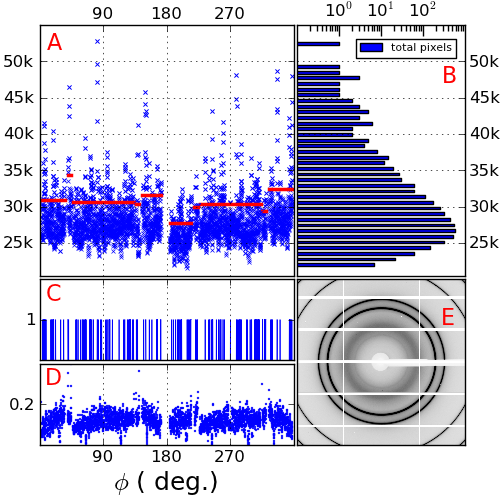
\includegraphics[ ]{./binary.png}
\end{center}
{\bf Figure 1} {\bf A)} Typical measurement of $n_{s}( q_{111},\phi)$, i.e. the photon counts around the Bragg ring at $q_{111}$. The horizontal bars show the binary cutoff along the ring for each module. {\bf B)} Histogram of the intensities in {\bf A} on a log scale of photon numbers. Notice the tail at higher intensities, indicating the presence of large particles. {\bf C)} Result of applying the binary filter to {\bf A}. A binary shot at $q_{111}$ is, on average, 10\% ones, 77\% zeros and 13\% masked pixels (masked pixels are ignored in the analysis).  {\bf D)} The average binary intensity from a scan of 500 snapshots. Notice how some of the regions are biased, indicating intra-module pixel variations. {\bf E)} Typical snapshot showing the Bragg rings at $q_{111}$ and $q_{200}$. Low/high intensities shown in white/black. \end{figure}


Data from 15,496 x-ray diffraction images of silver NP solution were collected and analyzed at the micro-focus crystallography beamline (12-2) at SSRL. We prepared a sample containing an estimated $10^{9}$  20 nm NPs per snapshot in the illuminated volume, but we observed significant numbers of NPs that were larger. Samples were loaded and oriented in the X-ray beam using the Stanford Automated Mounting System (SAM), controllable from the experimental hutch. Using a liquid nitrogen-cooled double crystal monochromator we tuned the beam energy to 17 keV. The beam was focused down to about $20 \times 50 \mu$ m$^2$ using Rh coated Kirkpatrick-Baez mirrors and had a flux of $2\cdot 10^{12}$ photons per second. Snapshots were recorded on a Dectris Pilatus 6M photon counting detector. 

To successfully measure a correlation function via the scheme (\ref{converge}), the sample must be frozen in time or space. Any random motion due to diffusion of particles will reduce the scattering correlation, which is a function of the particle structure and orientation (eq.~\ref{structurefactor}). To prevent diffusion during the long exposure times (order 1 second) necessary to scatter a sufficient number of photons to measure a correlation signal at a synchrotron, we cooled the sample using a 100 Kelvin nitrogen cryo jet, ensuring that the particles remained immobilized during each exposure. The silver NPs, coated in PVP, were synthesized following a protocol described elsewhere \cite{Levard:2011bx}. In order to prevent the formation of solvent crystals at the low temperature, the NPs were concentrated and suspended in 80\% glycerol and 3\% agarose with a final concentration of 350 mg/ml. The solutions were held in kapton capillaries (500 and 600 $\mu$m inner and outer diameter, respectively) and flash frozen in liquid nitrogen. Kapton and glycerol scatter into relatively lower angles, and we did not observe corruption of our silver NP signal with scattering from the kapton or glycerol. Samples were prepared a day early and stored in a liquid nitrogen bath. Further, no changes in the diffraction images were observed during the course of a single snapshot exposure, indicating the sample did not undergo significant diffusion or radiation damage.

Our goal was to record as many snapshots as possible, each one representing a different ensemble of particle orientations frozen in time. The sample holder was equipped to automatically rotate the capillary 150 degrees about its longitudinal axis, perpendicular to the beam. Photon counts were read out and reset every 0.7 second as the capillary rotated 0.3 degrees under continuous beam irradiation, yielding 500 shots per 150 degree rotational scan. This was deemed an optimal timing to simultaneously maximize signal and minimize damage and heating. Every 500 shots, between scans, the capillary was moved longitudinally so as to always probe different regions of the sample.

A bicubic interpolation algorithm was used to convert the cartesian pixel lattice to polar coordinates for calculation of (\ref{angular}). Using the Scherrer equation [8] relating the width of a Bragg ring to the average NP size, we concluded that the majority of silver NPs in each snapshot were roughly 20 nm in diameter. Histograms of photon counts into the $q_{111}$ Bragg ring indicate a rather large distribution of particle sizes (Figure 1-B) which we discuss in the following section.

\section{Results}


\begin{figure}
\label{fig:results}
\begin{center}
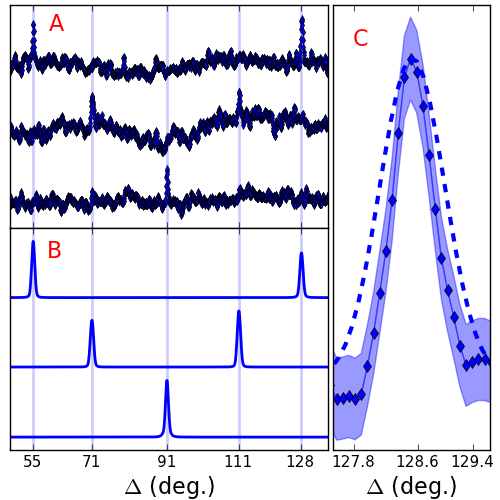
\includegraphics[ ]{./results.png}
\end{center}
{\bf Figure 2} {\bf A)} From top to bottom, 20 nm silver NP simulations of $D (q_{111},q_{200}, \Delta  )$, $D (q_{111},q_{111}, \Delta  )$, and $D (q_{200},q_{200}, \Delta  )$. {\bf B)} Corresponding measurements of the correlations plotted in {\bf A}. Vertical lines mark analytical predictions. We truncated the angular range to highlight the correlation peaks. The entire angular plot is symmetric about $\Delta = \pi$. Regions not shown contain artifacts similar to those on the figure, with nothing greater in magnitude than the CXS peaks. {\bf C)} Width of a correlation peak. The simulation was for 20 nm particles. Peak width scales inversely with particle size, hence we expect the measured CXS resulted from particles larger than 20 nm. Shading represents 95\% confidence intervals on the measurement.
\end{figure}

Here we report on our attempts to resolve (\ref{angular}) at the two brightest silver Bragg rings. Specifically, we calculated $D (q_{111},q_{111}, \Delta  )$, $D (q_{200},q_{200}, \Delta  )$, and $D (q_{111},q_{200}, \Delta  )$. 

Convergence of the CXS signal is complicated by the inherent statistical noises described in [1,7], and CXS measurement is sensitive to systematic noises associated with the experimental conditions \cite{Kam:1981ua}, \textit{e.g.}~detector artifacts. The Pilatus 6M detector is made up of 60 pixel modules separated by 1-2 mm gaps, and each Bragg ring subtends multiple modules. The overall electronic response of each module is slightly different, causing systemic anisotropies which lead to detector intensity correlations that dominate the sample CXS. 

To minimize the background correlations, we apply a binary filter to the data (Figure 1). We definea the filter as follows: Let $\{ \bm q_{hkl} \}_{m}$ represent the set of Bragg pixels on the $m^{th}$ detector module ($1 \leq m \leq 60$). Let $\mu_m$ and $\sigma_m$ represent the average and standard deviation of $n_{s}(\bm q)$  for all $\bm q \in \{ \bm q_{hkl} \}_{m} $, respectively. Then for each $\bm q \in \{ \bm q_{hkl} \}_{m} $, we apply the photon count filter:

\[  n_{s}(\bm q ) = 
 \begin{cases} 
   1 & \quad \text{if } n_{s}(\bm q ) > \mu_m +  \sigma_m\\
   0 & \quad \text{otherwise} 
 \end{cases} 
 \]

\textit{i.e.}~all pixels less than one standard deviation above the mean are set to zero and the rest are set to unity. The binary filter is a simple method for emphasizing the local variations from the sample compared to the background fluctuations of the detector; placing each detector module on the same scale removes correlations between modules.  After applying the filter and calculating (\ref{angular}), the resulting correlations reveal peaks that match the simulations and analytical predictions (Figure 2). Despite the filtering, variations remain within each module which bias the binary filter selection and lead to the low frequency background correlations seen in Figure 2-B. The binary filter is an intermediate stage in our on-going analysis; it provides a stepping stone to better data refinement techniques and CXS extraction.

As mentioned in the Methods section, we infer from the width of the Bragg rings that the majority of our sample consisted of $10^9$ 20 nm silver NPs. From tabulated coherent atomic cross sections \cite{Henke:1993wx} we estimated that each 20nm silver NP scattered roughly 1.6 photons per 0.7 sec exposure. We can further estimate that roughly 8.3\% of these NPs scatter into the Bragg ring at $q_{111}$ on the detector. This is done by tracing out volumes of rotation of the reciprocal lattice points whose diameter is given by the Scherrer equation [8], and then determining which fraction of that volume intersects the Ewald sphere. These estimates are in line with the average photon counts per pixel per snapshot that we observed in the $q_{111}$ Bragg ring, $\sim 4 \cdot10^4$. Many of the snapshots had Bragg peaks with counts $\sim 8 \cdot10^4$, much greater than one would expect given Poisson photon statistics. Thus we conclude that our sample included larger particles which scatter more photons. To put a lower bound on the size of these particles we again turned to the Scherrer equation, this time relating the width of the correlation peak to the particle size (Figure 2-C). We simulated (\ref{angular}) for 20 nm NPs and compared the widths of the simulated and measured correlation peaks. The width of the measured correlation peak is in line with estimates for 50 nm particles. Thus, we concluded that the correlations we are measuring are most likely generated by scattering off of thousands of $\ge$50 nm particles per shot. We emphasize that this is an estimated lower bound; effects not included in the Scherrer equation (e.g. Brownian motion) can cause broadening of a Bragg peak. We estimate that roughly 0.2\% of 50 nm silver NP orientations will simultaneously subtend 2 Bragg peaks on the detector at either $q_{111}$ or $q_{200}$.

We note that convergence of the correlations were not limited by the number of particles in the beam.  At present, the main impediment to accurate measurements of CXS arises from anisotropy artifacts induced by the detector system.  We have been able to partially overcome background correlations by nonlinear binary filtering and are continuing data processing with more sophisticated methods.

\section{Conclusion}

Kam's original results \cite{Kam:1977wc} show that (\ref{correlation}), which may be directly calculated from the structure factors of the particle (\ref{structurefactor}), can be derived from measurement of an ensemble of particles. Hence accurate measurement of CXS in the 3-dimensional $\{q_1,q_2,\Delta\}$ space can lead to constraints on a sample's electron density model, thus giving a route to iterative refinement \cite{Schroder:2010cm}. 

Our preliminary results reveal atomic scale information of the internal structure of a particle from a bulk sample containing many identical  but randomly oriented particles. These results on silver NPs suggest that it should be feasible to obtain atomic scale constraints on models of particles with unknown structures, provided one can effectively correct for background correlations. With the much brighter pulses from x-ray free electron lasers it may be possible to extend the results to more complex biomolecules \cite{Neutze:2000ih, Spence:2012eo}. 


\bibliographystyle{ieeetr}
%\bibliography{papers2.bib}
%
%
%
\begin{thebibliography}{10}

\bibitem{Kam:1977wc}
Z.~Kam, ``{Determination of macromolecular structure in solution by spatial
  correlation of scattering fluctuations},'' {\em Macromolecules}, vol.~10,
  no.~5, pp.~927--934, 1977.

\bibitem{Saldin:2011ch}
D.~Saldin, H.~Poon, M.~Bogan, S.~Marchesini, D.~Shapiro, R.~Kirian,
  U.~Weierstall, and J.~Spence, ``{New Light on Disordered Ensembles: Ab Initio
  Structure Determination of One Particle from Scattering Fluctuations of Many
  Copies},'' {\em Phys. Rev. Lett.}, vol.~106, p.~115501, Mar. 2011.

\bibitem{Kam:1981ua}
Z.~Kam, M.~H. Koch, and J.~Bordas, ``{Fluctuation x-ray scattering from
  biological particles in frozen solution by using synchrotron radiation.},''
  {\em Proceedings of the National Academy of Sciences}, vol.~78,
  pp.~3559--3562, June 1981.

\bibitem{Wochner:2009ia}
P.~Wochner, C.~Gutt, T.~Autenrieth, T.~Demmer, V.~Bugaev, A.~D. Ortiz, A.~Duri,
  F.~Zontone, G.~Gr{\"u}bel, and H.~Dosch, ``{X-ray cross correlation analysis
  uncovers hidden local symmetries in disordered matter.},'' {\em P Natl Acad
  Sci Usa}, vol.~106, pp.~11511--11514, July 2009.

\bibitem{Kam:1985tz}
Z.~Kam and I.~Gafni, ``{Three-dimensional reconstruction of the shape of human
  wart virus using spatial correlations.},'' {\em Ultramicroscopy}, vol.~17,
  no.~3, pp.~251--262, 1985.

\bibitem{Starodub:1fy}
D.~Starodub, A.~Aquila, S.~Bajt, M.~Barthelmess, A.~Barty, C.~Bostedt, J.~D.
  Bozek, N.~Coppola, R.~B. Doak, S.~W. Epp, B.~Erk, L.~Foucar, L.~Gumprecht,
  C.~Y. Hampton, A.~Hartmann, R.~Hartmann, P.~Holl, S.~Kassemeyer, N.~Kimmel,
  H.~Laksmono, M.~Liang, N.~D. Loh, L.~Lomb, A.~V. Martin, K.~Nass, C.~Reich,
  D.~Rolles, B.~Rudek, A.~Rudenko, J.~Schulz, R.~L. Shoeman, R.~G. Sierra,
  H.~Soltau, J.~Steinbrener, F.~Stellato, S.~Stern, G.~Weidenspointner,
  M.~Frank, J.~Ullrich, L.~S.~u. der, I.~Schlichting, H.~N. Chapman, J.~C.~H.
  Spence, and M.~J. Bogan, ``{Single-particle structure determination by
  correlations of snapshot X-ray diffraction patterns},'' {\em Nature
  Communications}, vol.~3, pp.~1276--7, 1.

\bibitem{Elser:2011ez}
V.~Elser, ``{Strategies for processing diffraction data from randomly oriented
  particles},'' {\em Ultramicroscopy}, vol.~111, pp.~788--792, June 2011.

\bibitem{Liu:2013dv}
H.~Liu, B.~K. Poon, D.~K. Saldin, J.~C.~H. Spence, and P.~H. Zwart,
  ``{Three-dimensional single-particle imaging using angular correlations from
  X-ray laser data},'' {\em Acta Crystallogr A Found Crystallogr}, vol.~69,
  pp.~365--373, May 2013.

\bibitem{Chen:2013io}
G.~Chen, P.~H. Zwart, and D.~Li, ``{Component Particle Structure in
  Heterogeneous Disordered Ensembles Extracted from High-Throughput Fluctuation
  X-Ray Scattering},'' {\em Phys. Rev. Lett.}, vol.~110, p.~195501, May 2013.

\bibitem{Saldin:2009jj}
D.~K. Saldin, V.~L. Shneerson, R.~Fung, and A.~Ourmazd, ``{Structure of
  isolated biomolecules obtained from ultrashort x-ray pulses: exploiting the
  symmetry of random orientations},'' {\em J. Phys.: Condens. Matter}, vol.~21,
  p.~134014, Mar. 2009.

\bibitem{Saldin:2010bx}
D.~K. Saldin, H.~C. Poon, V.~L. Shneerson, M.~Howells, H.~N. Chapman, R.~A.
  Kirian, K.~E. Schmidt, and J.~C.~H. Spence, ``{Beyond small-angle x-ray
  scattering: Exploiting angular correlations},'' {\em Phys. Rev. B}, vol.~81,
  p.~174105, May 2010.

\bibitem{Poon:2013ia}
H.~C. Poon, P.~Schwander, M.~Uddin, and D.~K. Saldin, ``{Fiber Diffraction
  without Fibers},'' {\em Phys. Rev. Lett.}, vol.~110, p.~265505, June 2013.

\bibitem{Kurta:2012cb}
R.~P. Kurta, M.~Altarelli, E.~Weckert, and I.~A. Vartanyants, ``{X-ray
  cross-correlation analysis applied to disordered two-dimensional systems},''
  {\em arXiv}, Feb. 2012.

\bibitem{Kurta:2013to}
R.~P. Kurta, M.~Altarelli, and I.~A. Vartanyants, ``{X-ray cross-correlation
  analysis of disordered systems: potentials and limitations},'' {\em arXiv},
  Feb. 2013.

\bibitem{Kirian:2011bq}
R.~A. Kirian, K.~E. Schmidt, X.~Wang, R.~B. Doak, and J.~C.~H. Spence,
  ``{Signal, noise, and resolution in correlated fluctuations from snapshot
  small-angle x-ray scattering},'' {\em Phys. Rev. E}, vol.~84, p.~011921, July
  2011.

\bibitem{Levard:2011bx}
C.~Levard, B.~C. Reinsch, F.~M. Michel, C.~Oumahi, G.~V. Lowry, and G.~E.
  Brown, Jr., ``{Sulfidation Processes of PVP-Coated Silver Nanoparticles in
  Aqueous Solution: Impact on Dissolution Rate},'' {\em Environ. Sci.
  Technol.}, vol.~45, pp.~5260--5266, June 2011.

\bibitem{Henke:1993wx}
B.~L. Henke, E.~M. Gullikson, and J.~C. Davis, ``{X-Ray Interactions:
  Photoabsorption, Scattering, Transmission, and Reflection at E= 50-30,000 eV,
  Z= 1-92},'' {\em Atomic data and nuclear data tables}, 1993.

\bibitem{Schroder:2010cm}
G.~F. Schr{\"o}der, M.~Levitt, and A.~T. Brunger, ``{Super-resolution
  biomolecular crystallography with low-resolution data},'' {\em Nature},
  vol.~464, pp.~1218--1222, Apr. 2010.

\bibitem{Neutze:2000ih}
R.~Neutze, R.~Wouts, D.~van~der Spoel, E.~Weckert, and J.~Hajdu, ``{Potential
  for biomolecular imaging with femtosecond X-ray pulses.},'' {\em Nature},
  vol.~406, pp.~752--757, Aug. 2000.

\bibitem{Spence:2012eo}
J.~C.~H. Spence, U.~Weierstall, and H.~N. Chapman, ``{X-ray lasers for
  structural and dynamic biology},'' {\em Rep. Prog. Phys.}, vol.~75,
  p.~102601, Sept. 2012.

\end{thebibliography}

%
%
% new refs to be added
\end{document}






